%%%%%%%%%%%%%%%%%%%%%%%%%%%%%%%%%%%%%%%%%%%%%%%%%%%%%%%%%%%%%%%%%%%%%%%%%%%%%%%%
%2345678901234567890123456789012345678901234567890123456789012345678901234567890
%        1         2         3         4         5         6         7         8

\documentclass[letterpaper, 10 pt, conference]{ieeeconf}  % Comment this line out
                                                          % if you need a4paper
%\documentclass[a4paper, 10pt, conference]{ieeeconf}      % Use this line for a4
                                                          % paper

\IEEEoverridecommandlockouts                              % This command is only
                                                          % needed if you want to
                                                          % use the \thanks command
\overrideIEEEmargins
% See the \addtolength command later in the file to balance the column lengths
% on the last page of the document



% The following packages can be found on http:\\www.ctan.org
%\usepackage{graphics} % for pdf, bitmapped graphics files
%\usepackage{epsfig} % for postscript graphics files
%\usepackage{mathptmx} % assumes new font selection scheme installed
%\usepackage{times} % assumes new font selection scheme installed
\usepackage{amsmath} % assumes amsmath package installed
%\usepackage{amssymb}  % assumes amsmath package installed
\usepackage{graphicx}

\DeclareMathOperator*{\argmin}{arg\,min}

\newcommand{\norm}[1]{\left\lVert#1\right\rVert}

\title{\LARGE \bf
Machine Learning, Project 2: Text Classification for Sentiment Analysis}

%\author{ \parbox{3 in}{\centering Huibert Kwakernaak*
%         \thanks{*Use the $\backslash$thanks command to put information here}\\
%         Faculty of Electrical Engineering, Mathematics and Computer Science\\
%         University of Twente\\
%         7500 AE Enschede, The Netherlands\\
%         {\tt\small h.kwakernaak@autsubmit.com}}
%         \hspace*{ 0.5 in}
%         \parbox{3 in}{ \centering Pradeep Misra**
%         \thanks{**The footnote marks may be inserted manually}\\
%        Department of Electrical Engineering \\
%         Wright State University\\
%         Dayton, OH 45435, USA\\
%         {\tt\small pmisra@cs.wright.edu}}
%}

\author{
  Jeanne Chaverot, Etienne Caquot, Aslam Cader \\
  \textit{Department of Computer Science, EPFL, Switzerland}
}


\begin{document}

\maketitle
\thispagestyle{empty}
\pagestyle{empty}


%%%%%%%%%%%%%%%%%%%%%%%%%%%%%%%%%%%%%%%%%%%%%%%%%%%%%%%%%%%%%%%%%%%%%%%%%%%%%%%%
\begin{abstract}

The goal of this project is to predict if a tweet message used to contain a positive :) or negative :( smiley by considering only the remaining text, as the smileys (labels) have been removed from the tweets. In this project, we have tried to implement as many different models as possible to have a general view of machine learning techniques for text classification.

\end{abstract}


%%%%%%%%%%%%%%%%%%%%%%%%%%%%%%%%%%%%%%%%%%%%%%%%%%%%%%%%%%%%%%%%%%%%%%%%%%%%%%%%
\section*{INTRODUCTION}

This problem is a binary classification problem with text. Thus, we will follow NLP (Natural Language Processing) methods to classify these tweets as accurately as possible.
The first main part of the project is the text pre-processing. Although the input data (positive, negative and test tweets) has already been pre-processed, we have continued the operation, which we explain in Section~\ref{sec:preprocess}. 
In Section~\ref{sec:models}, we comment on the different text classification models we have implemented and discuss their strengths and weaknesses. 
We describe our results in Section~\ref{sec:results} and conclude in Section~\ref{sec:conclusion}

\section{Data pre-processing}
\label{sec:preprocess}

The data we were given had already been prepared, words and punctuation are properly separated by a white-space.

Pre-processing tweets can be tricky as each user is free to write as he/she wants. Our data-set contains grammar mistakes/typos, words exaggerations ("\textit{heyyy duuude}" instead of "\textit{hey dude}"), slang, irony (which ironically is shown with the use of emojis), shortcuts. 
There are several ways to deal with text, and we present how we dealt with these issues and note whether it has improved or not the accuracy of our models.

\subsection{Data pre-processing that penalized our classifiers}
\begin{itemize}
    \item Remove stop-words \ \\
    Stop-words are very frequent words that carry very small information. 
    We removed them from our set of tweets. Our initial hypothesis was that stop-words don't bring any information to our model but added some complexity to it (as they increase the vocabulary size). However, after removing the stop-words we observed a decrease in our models' accuracy.
    Indeed, some of the models we used (e.g. LSTM) try to understand the whole meaning of each tweet by analyzing its context.\vspace*{0,25\baselineskip}
    \item Lemmatize \ \\
    Lemmatization is the action of stemming and mapping words with a predefined lexicon. Stemming is to bring together words that have different forms but the same meaning (\textit{eg.: study, studying, studied} become \textit{study}).
    As for the stop-words, we thought that lemmatizing our tweets would allow us to bag words together and reduce the models' complexity. However, after the lemmatization, our models' accuracy decreased.
    One of the hypotheses to explain this is that by putting together some words, we generalize them and lose some precision.
\end{itemize}

\subsection{Data pre-processing that were efficient}
\begin{itemize}
    \item Remove numbers \ \\
    Since our analysis is to determine whether a tweet supposedly contained a :) or a :(, numbers are not relevant. Indeed, they do not express any sentiment and can't be considered as a positive or negative value. Removing it will reduce complexity (bag word size will diminish).\vspace*{0,25\baselineskip}
    \item Remove users and URLs \ \\ 
    We have removed the user and URL tags as they do not bring information to the corpus.\vspace*{0,25\baselineskip}
    \item Create positive and negative sets of words. \ \\
    We had an initial hypothesis that the most common words appearing in the positive (respectively negative) tweets gave a lot of information about the label of a tweet. Therefore, we have selected all the words among the 1000 most common words that appear at least 80\% of the time in the positive (respectively negative) set and translated those words to "good" (respectively "bad"). This way, we reduce the vocabulary length, strengthen the influence of such words and fasten our model.
    \vspace*{0,5\baselineskip}

   
    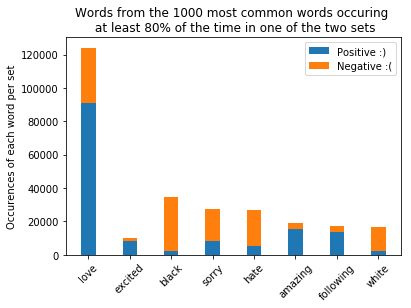
\includegraphics[width=0.45\textwidth]{histogram_ML.png}
    

    For instance, the word \textit{amazing} has been replaced by \textit{good} in all tweets, as we've seen that at least 80\% of the tweets it appears in are positive. Similarly, every occurrence of the word \textit{sorry} has been replaced by \textit{bad}.\vspace*{0,25\baselineskip}
    
    \item Remove the least common terms \ \\
    We have retrieved all the terms that appear at most five times in the training set and removed them from the tweets. These represent more than 400'000 words that have been taken out of our vocabulary. We removed them as they can't be used by the model to predict a tweet's label (not enough occurrences).
\end{itemize}


\section{Models}
\label{sec:models}
In this section, we will present the various machine learning models we used during this project. As we will see in section~\ref{sec:results}, those models lead to very contrasting results.

\subsection{Logistic Regression with GloVe embedding}
\label{subsec:Glove}

In the project README, there was a description of the steps to build a text classifier. This model is the implementation of those steps. We were given bash scripts that we ran and they provided us the vocabulary and the Co-occurrence matrix of the words in our corpus of tweets. In this process, we ignore words that appear less than 5 times. Given now the vocabulary and the Co-occurrence matrix we performed the GloVe~\cite{pennington2014glove} algorithm and obtain embedding for our word. Now that we have an embedding for each word, we embed a tweet by averaging the embedding of each word in this tweet. That is for a tweet $t$ we compute its embedding as $\frac{1}{|t|} \sum_{w_i \in t} w_i$, with $w_i$ the embedding of word $i$ in the tweet $t$. Now that we have an embedding for each of our tweets, we can perform a binary classification task using Logistic Regression. We used the scikit-learn library~\cite{scikit-learn}. The aim of penalized logistic regression is to find $w$ that minimizes the following:
$$ \argmin_w \sum_{n=1}^{N} \ln{(1+\exp{(\boldsymbol{x_n}^T\boldsymbol{w})})} - y_n\boldsymbol{x_n}^T\boldsymbol{w} + \lambda \norm{\boldsymbol{w}}^2  $$
We used 4-fold Cross-Validation with simple Grid-Search to find the optimal regularization hyper-parameters $\lambda$ to train our model. We used a sag solver.

\subsection{Logistic Regression with Word2vec embedding}

In this approach, we use the Word2vec~\cite{2013arXiv1301.3781M} models to create an embedding from our tweets. The Word2vec models are neural networks with two layers which aim at reconstructing the linguistic context of a word. It takes text as input and produces a vector space, with each word having representation in this vector space. We used a python library that provides an interface to Google Word2vec~\cite{word2vec}. We ignored the words that appear less than 5 times in the tweets. Finally, as in the first approach, we average the embedding of the words in the tweets to obtain an embedding for each tweet. Once we have the embedding for our tweets, we perform a supervised classification task using a Logistic Regression and used the same process as in subsection~\ref{subsec:Glove} to optimize the classifier.

\subsection{VADER} 

 This model uses VADER (\textbf{V}alence \textbf{A}ware \textbf{D}ictionary for s\textbf{E}ntiment \textbf{R}easoning)~\cite{vader}, which is a simple rule-based model for general sentiment analysis. Vader is part of the well-known python package for Natural Language Processing NLTK~\cite{nltk}. There is no training task in this model, we could directly plug our test set as input to VADER and it will associate 3 probabilities to each tweet in our test set. The 3 probabilities would sum to 1 and be strictly positive. For each tweet, VADER will evaluate the sentiment of the tweet and will give a probability for the tweet being \textit{positive / neutral / negative}. With those values, we can then threshold the values to either class our tweets as positive or negative.

\subsection{MonkeyLearn} 

MonkeyLearn is an online web-service that provides text analysis models through an API. They have a Sentiment Analysis model and when querying with some tweets seemed to predict correctly. Unfortunately, the free plan allows to do only 300 queries per month. We ended up abandoning this solution.

\subsection{LSTM (Long Short-Term Memory) } 

LSTM is a neural network, which is part of what is called Recurrent Neural Networks (RNN). LSTM has memory cells in its architecture which enables the neural network to "remember" the word that has been seen before the one that is being processed. This memory cell is particularly suited for text processing because a word is part of a sentence and can have different meanings in different contexts. For instance, the word "dog" won't have the same meaning if it is preceded by "hot" or not. We used the library Keras~\cite{chollet2015keras} to construct our Neural Network. We have created three layers, one is an embedding layer, followed by an LSTM layer and finally a dense layer. 

Before the embedding layer, we used a tokenizer to create a vocabulary from our tweets. In this vocabulary the most common word will be at index 1, the second most frequent will have index 2, etc...). We ignore words that appear less than five times in the tweets. Each tweet will be represented by the sequence of indexes of the words in it. The maximum number of words in a tweet was 46, we choose to pad each sequence with zeros to have all sequences of length 50. 

Now we can pass our sequences to the embedding layer which will associate to each value in a sequence an embedding of dimension 300. Hence, this layer has 300 cells. Now our tweets are represented by a matrix of dimension 50X300. 

Then comes the LSTM layer, we decided that this layer would have 256 cells which was the closest power of 2 smaller than 300. We set the recurrent dropout of 0.2 to avoid overfitting our data. This layer has 2 activation functions : hyperbolic tangent for the outputs and sigmoid for the feedback path.

Finally comes our last layer that is a dense layer with 1 cell. This layer has a sigmoid as activation function. This will produce outputs between 0 and 1 for each tweet, we can now threshold back to -1 or 1. Note than we associated the value 0 to negative tweets and value 1 to positive tweets in our training set. We used binary cross-entropy as our loss function and an Adam optimizer.

\subsection{Google BERT or the beast of the classifier}
    
\textbf{B}idirectional \textbf{E}ncoder \textbf{R}epresentations from \textbf{T}ransformers (BERT) is an open-source pre-trained model from Google. It has been mainly designed for Natural Language Processing (NLP) tasks. This model is mainly known to beat all the other state-of-the-art NLP systems.

It can be used for many tasks such as question/answer tasks (SQuAD), summarizing, classification among others. 

BERT\cite{BERT_paper} is, at first, an unsupervised model that has been pre-trained with millions of sentences (Wikipedia and Book Corpus). We use this pre-trained model and fine-tuned it with our data set. 
The model we used is BERT-Base, the Uncased one because tweets have been lowercased. This model is a neural network that contains 12-layer, 768-hidden, 12-heads, 110M parameters.
This model needs the text to be of fixed length. Since a tweet size is limited (max 280 characters), BERT can easily bound its size and add padding as we did with LSTM.

BERT uses sentencepiece (an unsupervised text tokenizer library) to pre-process the data. Each sentence is tokenized, and tags are added in the sentence: one at the beginning \textit{[CLS]} and one at the end \textit{[SEP]}). The model needs these separators to put delimitation on the text. 
This tokenizer is not language-dependent and uses a WordPiece model: it means that a word can be split into sub words and also characters (e.g.: \textit{embeddings} becomes \textit{['em', '\#\#bed', '\#\#ding', '\#\#s']}). The hashtags added during the tokenization allow knowing that there are sub words beforehand. 
This segmentation is done to obtain a fixed final vocabulary size, optimized for Neural Text Processing \cite{BERT_preprocessing}. 

Once the pre-processing is done, fine-tuning can be performed. We decided to split the dataset as follows: 80\% for the training set and 20\% for the test set to optimize the loss. To fine-tune the model in a reasonable amount of time, we needed to have access to several high-performance GPUs or TPUs (takes several hours with an Nvidia Tesla P100).

Compared to other models, BERT is more accurate because the representation is done deeply bidirectionally. It means that it deeply understands words within a context (since a word can have a semantically different meaning depending on how it is used) \cite{BERT_paper}: BERT can understand the difference of the meaning of the word \textit{'right'} in \textit{'This person is right'} and \textit{'Turn right at the end of the road'}. In opposite to that, our previous models GloVe and Word2vec are context-free models and do not differentiate them. 

\section{Results}
\label{sec:results}

This section details the results of our models presented in Section~\ref{sec:models}.

\subsection{Logistic Regression with GloVe embedding} 

With the scripts that were given and Logistic Regression, we could reach an accuracy of 72\%. Seeing it was difficult to improve this score, we rapidly switched to a new embedding algorithm Word2vec.
  
\subsection{Logistic Regression with Word2vec embedding} 
  
With Word2vec embedding, we managed to reach an accuracy of 77\%. We explain this increase from GloVe because Word2vec uses neural networks to create embedding. We also started to understand that we should increase the size of our embedding that we didn't do with GloVe.

\subsection{VADER} 
We had high hopes in VADER, it was kind of magic. The algorithm did not require any training, and we just had to prepossess the tweets with the NLTK methods. It turns out there is no magic in the Machine Learning world and VADER was very bad at predicting sentiment for our tweets. Most of the time we had a high probability of Neutral sentiment in the tweet. Which is not helpful to our project. The best accuracy score we reached with VADER is 63\%. 

\subsection{LSTM (Long Short-Term Memory)} 

With LSTM, the best score we could achieve is 84.7\%. To do so we needed to avoid overfitting. With Keras, we could implement Early Stopping: this method consists in stopping the training when the validation loss starts to increase. We split our training data into 80\% training and 20\% validation and at the end of each epoch, we evaluate the loss on the validation set. If for 5 epoch the validation loss increases then we stop the training and keep the model with the best validation loss. The next graph shows the evolution of training and validation loss.

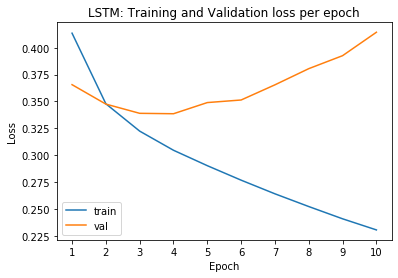
\includegraphics[width=0.45\textwidth]{train_val_accuracy.png}
Here the model we kept would be the one after epoch 4. 


\subsection{Google BERT or the beast of the classifier}

The best accuracy we achieved with BERT is \textbf{88.2\%}. Here are the parameters used to obtain this result:
\begin{itemize}
    \item epoch = 3
    \item batch\_size = 16
    \item learning\_rate = 2e-5 
\end{itemize}{}

This result was obtained by using the dataset without any pre-processing. Indeed, by doing our pre-processing step with the same parameters, we obtained an accuracy of 85.7\%. As explained before, BERT uses every little hint on text to learn something, and by generalizing or removing any element, we remove the information and reduce the accuracy of our model. Moreover, BERT uses its own pre-processing that is adapted for the bidirectional encoding of the model.

Unfortunately, fine-tuning being computationally expensive, we weren't able to find the optimal parameter to obtain the best accuracy. Fortunately, we were able to use Colab (by Google), an online python notebook, in which we can use a cloud GPU/TPU. We were allocated either an Nvidia Tesla P4 or P100. We were lucky when we had the latter because it's 2.4 times faster than the first one and 7 times faster than an Intel i7-3930k (CPU). However, training still took several hours.


\subsection{Comparison of Accuracies}
Here is a visual comparison of our models and the accuracies we have obtained for each one of them. BERT has been the most successful model, achieving an accuracy of 88.2\%, followed by the LSTM with 84.7\%.

\begin{table}[!htbp]
    \centering

\begin{tabular}{|c||c|c|}\hline
%%%%%% Title row starts here
Model & Best Accuracy  \\ \hline\hline
%%%%%% Row Foo starts here
Logistic Regression with GloVe embeddings &
\begin{tabular}{c} 72\% \\
\end{tabular}\\ \hline
%%%%%% Row Foo starts here
Logistic Regression with Word2Vec embeddings &
\begin{tabular}{c} 77\% \\
\end{tabular}\\ \hline
%%%%%% Row Bar starts here
VADER &
\begin{tabular}{c} 63\% \\
\end{tabular}\\ \hline
%%%%%% Row Bar starts here
LSTM &
\begin{tabular}{c} 84.7\% \\ 
\end{tabular}\\ \hline
%%%%%% Row Bar starts here
BERT &
\begin{tabular}{c} 88.2\% \\ 
\end{tabular}\\ \hline 

\end{tabular}
\caption{Best accuracy obtained per model}
\end{table}

\section{Conclusion}
\label{sec:conclusion}
It’s really difficult to teach a machine to understand any text when a person’s writing is unpredictable. 
This tweet classification problem presented us most of the issues we might face while dealing with text. Pre-processing, in general, is an important step where we have to make pertinent choices to avoid penalizing our model. Pre-processing text is challenging since we need to analyze and determine whether a specified technique can optimize or not the classifier. Such decisions depend on the data we’re working with: we won’t deal with scientific papers the same way we’re dealing with tweets. 
Finding the best classifier was more than a challenge since for each of them, we had to understand how it works and do a ‘grid-search’ like experiment to denote which one is optimal for our problem. It’s really interesting to see every approach and how the models try to understand the tweets.
Bert ended up being the best-fit for this problem because it combines different models' techniques and uses a bidirectional representation. 
But the more complicated the model gets, the more computationally expensive it becomes, and we noticed that we also need good GPUs/TPUs if we want to train our models in a reasonable amount of time.

\addtolength{\textheight}{-12cm}   % This command serves to balance the column lengths
                                  % on the last page of the document manually. It shortens
                                  % the textheight of the last page by a suitable amount.
                                  % This command does not take effect until the next page
                                  % so it should come on the page before the last. Make
                                  % sure that you do not shorten the textheight too much.

%%%%%%%%%%%%%%%%%%%%%%%%%%%%%%%%%%%%%%%%%%%%%%%%%%%%%%%%%%%%%%%%%%%%%%%%%%%%%%%%



%%%%%%%%%%%%%%%%%%%%%%%%%%%%%%%%%%%%%%%%%%%%%%%%%%%%%%%%%%%%%%%%%%%%%%%%%%%%%%%%



%%%%%%%%%%%%%%%%%%%%%%%%%%%%%%%%%%%%%%%%%%%%%%%%%%%%%%%%%%%%%%%%%%%%%%%%%%%%%%%%


%%\begin{thebibliography}{99}

%%bibitem{c1} C. N. Fischer, R. K. Cytron \& R. J. LeBlanc. ÒCrafting a CompilerÓ, 2nd ed.,Boston: Pearson Education, 2010.

%%\end{thebibliography}

\bibliographystyle{ieeetr}
\bibliography{literature.bib}

\end{document}
